%\section{Using equations} 

 \begin{center}
\line(1,0){300} %\line(1,0){250}
\end{center}

\section*{Homework}

\noindent \textbf{Start by doing Practice exercises \#1-4 in the workbook.}

\bigskip
 
\noindent \textbf{Do you know \ldots}

\begin{itemize}
\item What it means to ``evaluate'' a function? 
\item Why some numbers are underlined in our calculation?
\item How to evaluate an function when the independent variable occurs more than once? 
\item How to generate a table or graph from an equation? 
\item What graphs of different types of functions look like? 
\item What a power, polynomial, or quadratic equation look like?
\item[~] \textbf{If you're not sure, work the rest of exercises and then return to these questions.  Or, ask your instructor or a classmate for help.} 
\end{itemize} 

\subsection*{Exercises}

\begin{enumerate} 
\setcounter{enumi}{4}

\item The 2002 Chevrolet Tahoe 4WD will take about 158.1 feet to stop when traveling at 60 mph in normal highway conditions.  Let $S$ be the speed at which the vehicle is traveling, in miles per hour (mph), and $D$ the distance it takes to stop, in feet.  This information together with a little physics gives the equation $$D = .0439S^2 + 1.47S$$
\begin{enumerate}
\item According to this equation, how many feet does it take to stop the Tahoe when traveling 80 miles per hour?
\item In driver's training classes they teach the ``two-second rule'' for safety:  you should follow no closer than two seconds behind the car in front of you.  If you are traveling 80 miles per hour, how many feet can you travel in two seconds?  \emph{Hint: convert to feet per second, then multiply by two seconds.}
\item Compare your results from parts (a) and (b) to decide if the ``two-second rule'' is adequate for safety at 80 miles per hour.  That is, if you are following two seconds behind the car in front of you and calamity strikes that car, will you be able to stop before hitting it?
\item Is the ``two-second rule'' adequate at 50 mph?
\end{enumerate}

\item Mom always said to sit close to the lamp when I was reading.  The intensity of light $L$, measured in percentage (\%) that you see from a lamp depends on your distance from the lamp, $F$ feet as described by the formula $$L=\frac{100}{F^2}$$
 \hfill \emph{Story also appears in 1.1 and 3.3 Exercises}
\begin{enumerate}
\item Calculate the  intensity when I sit 1 foot, 2 feet, or 3 feet away.
\item The other day I was sitting 27 inches from the lamp. What was the intensity of the light there? 
\item Calculate the rate of change of light intensity between 2 feet and 27 inches.  What does that tell you in terms of the story?
\item Draw a graph illustrating the function.
\end{enumerate}

\item Urban community gardens are catching on.  What was once an abandoned lot down the block is now a thriving 10'$\times$25' vegetable and berry garden for the neighborhood. (Remember ' stands for ``feet,'' so the garden is 10 feet wide and 25 feet long.)  One neighbor volunteered to donate gravel to make a path around the garden.  The path will be 3 inches deep and the same width all around. 
\begin{center}
\scalebox {.4} {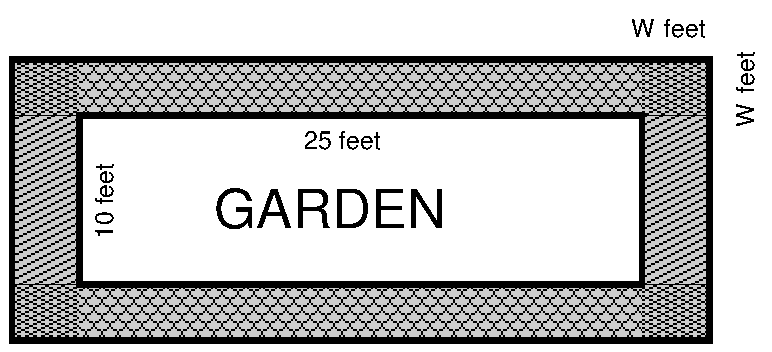
\includegraphics{GravelPath.pdf}}
\end{center}
 \hfill \emph{Story also appears in 2.4 Exercises and 3.5 \#4}
\begin{enumerate}
\item The other measurements are in feet, so convert the depth of the path (3 inches) into feet also.  
\item Suppose for the moment that the path will be 4 feet wide. Calculate the area of the path.  Here's one way to do it:  first, find the area of the outer rectangle, then subtract the area of the garden itself.

\emph{Hint:  the length of that outer rectangle includes the 25 feet of garden plus the width of the path on each side.   Same for the width of that outer rectangle.}
\item Figure out how much gravel they would need  (in cubic feet) for a 4 foot wide path by multiplying your answers to (a) and (b). 
\item  Actually, they aren't sure how wide the path should be and how much gravel they can get.  Let's write $W$ = width of path (feet) and $G$ = amount of gravel (cubic feet).  It turns out that $$G = W^2 + 17.5W$$
Check that when you evaluate at $W=4$ you get the same answer as in (c).
\item How many cubic feet of gravel would they need to make the path 2 feet wide? 3 feet wide?  42 inches? 
\end{enumerate}

\item One measure of the diversity of our news source is the count of the number of different daily newspapers in circulation.  A reasonable equation estimating this count over the past century is $$N = -.0021T^3+.34T^2-20T+ \text{2,226}$$ where $N$ is the number of daily newspapers in circulation in the United States $T$ years after 1900.
\begin{enumerate}
\item Based on this equation, how many daily newspapers were in circulation in 1920?  In 1955?  In 1995?  In 2010?
\item During which period were the number of newspapers in circulation dropping faster:  1900 to 1920 or 1995 to 2010?
\item Draw a graph illustrating the dependence.
\end{enumerate}

\item Mrs.\ Weber's cooking class came up with the equation $$M = 1.2F^2+4F+7$$ to approximate the grilling time of a piece of fish depending on its thickness.  Here $M$ is the number of minutes to grill the fish and $F$ is the thickness of the fish (in inches).  

\hfill \emph{Story also appears in 1.1 and 3.5 Exercises}
\begin{enumerate}
\item Evaluate the equation at $F=.25, 1, 1.5,$ and $2$.
\item What do the answers you found say about cooking fish?
\item Draw a graph showing how the cooking time depends on the thickness of the fish.
\item Your graph should show that the function is increasing.  Explain how that makes sense in terms of the story.
\end{enumerate} 

\item Wynter has a pretty decent job. He is paid a salary of \$780 per week but his hours vary week-to-week. Even though Wynter is not paid by the hour, he can figure out what his hourly wage would be depending on the number of hours he works.  For example, in a week where Wynter works 40 hours, he's earning the equivalent of \$19.50/hr because $$\frac{\$780}{40 \text{ hours}} = 780 \div 40 =\$19.50\text{/hour}$$

\hfill \emph{Story also appears in 3.3 Exercises}
\begin{enumerate}
\item What's Wynter's equivalent hourly wage in a week when he works 50 hours? 60 hours?
\item Name the variables and write an equation relating them.
\item Explain why this function is decreasing.
\end{enumerate} 


\end{enumerate}
